\documentclass[../main/main.tex]{subfiles}

\newdate{date}{10}{12}{2020}

% \begin{figure}[h!]
% \centering
% \includegraphics[page=6,width=0.8\textwidth]{../lessons/pdf_file/24_lecture.pdf}
% \end{figure}

%\displaydate{date}. Compiled:  \today. Alice.

\begin{document}

\pagestyle{plain}

\section{Lecture 24}


\subsubsection*{Slide 1}

\begin{minipage}[]{0.5\linewidth}
\centering
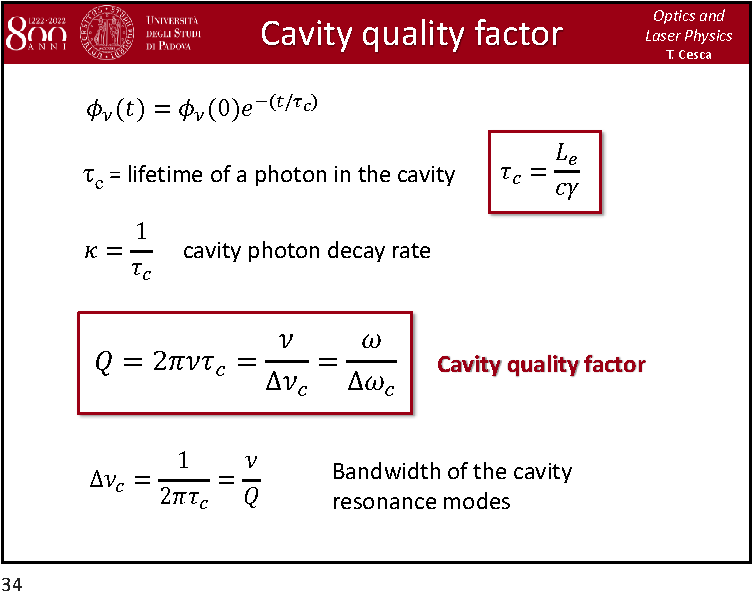
\includegraphics[page=1,width=1\textwidth]{../lessons/pdf_file/24_lecture.pdf}
\end{minipage}
\hspace{0.3cm}\vspace{0.3cm}
\begin{minipage}[c]{0.47\linewidth}

The cavity is a key aspect for realizing a laser. We have already introduced these quantities.


\end{minipage}

\subsubsection*{Slide 2}

\begin{minipage}[]{0.5\linewidth}
\centering
\includegraphics[page=2,width=1\textwidth]{../lessons/pdf_file/24_lecture.pdf}
\end{minipage}
\hspace{0.3cm}\vspace{0.3cm}
\begin{minipage}[c]{0.47\linewidth}

How can we move these concepts in the nanoscale world? Let us have a nanoscale cavity. We have an atom inside the cavity which can be schematized as a two-level system.

The interaction among the atom and the cavity is controlled by the three paramaters \( k, \, \Gamma, \, g_0  \).

We have the condition for \textbf{weak} and \textbf{strong} coupling. Also in the macroscopic world the interaction between these two regime is quite large.

\end{minipage}

\subsubsection*{Slide 3}

\begin{minipage}[]{0.5\linewidth}
\centering
\includegraphics[page=3,width=1\textwidth]{../lessons/pdf_file/24_lecture.pdf}
\end{minipage}
\hspace{0.3cm}\vspace{0.3cm}
\begin{minipage}[c]{0.47\linewidth}

\end{minipage}

\newpage

\subsubsection*{Slide 4}

\begin{minipage}[]{0.5\linewidth}
\centering
\includegraphics[page=4,width=1\textwidth]{../lessons/pdf_file/24_lecture.pdf}
\end{minipage}
\hspace{0.3cm}\vspace{0.3cm}
\begin{minipage}[c]{0.47\linewidth}

\end{minipage}

\subsubsection*{Slide 5}

\begin{minipage}[]{0.5\linewidth}
\centering
\includegraphics[page=5,width=1\textwidth]{../lessons/pdf_file/24_lecture.pdf}
\end{minipage}
\hspace{0.3cm}\vspace{0.3cm}
\begin{minipage}[c]{0.47\linewidth}

\end{minipage}

\subsubsection*{Slide 6}

\begin{minipage}[]{0.5\linewidth}
\centering
\includegraphics[page=6,width=1\textwidth]{../lessons/pdf_file/24_lecture.pdf}
\end{minipage}
\hspace{0.3cm}\vspace{0.3cm}
\begin{minipage}[c]{0.47\linewidth}

This is the most difficult parameter to calculate. It depends on the kind of transition you are considering. It is inverse proportional to the volume of the mode inside the cavity.

\end{minipage}

\newpage

\subsubsection*{Slide 7}

\begin{minipage}[]{0.5\linewidth}
\centering
\includegraphics[page=7,width=1\textwidth]{../lessons/pdf_file/24_lecture.pdf}
\end{minipage}
\hspace{0.3cm}\vspace{0.3cm}
\begin{minipage}[c]{0.47\linewidth}

If we assume that \( k > \Gamma  \), in order to be in the \textbf{strong coupling} regime we can obtain a condition for the quality factor. So, it is not that easy to be in this regime, we have stringent condition to satisfy.

\end{minipage}

\subsubsection*{Slide 8}

\begin{minipage}[]{0.5\linewidth}
\centering
\includegraphics[page=8,width=1\textwidth]{../lessons/pdf_file/24_lecture.pdf}
\end{minipage}
\hspace{0.3cm}\vspace{0.3cm}
\begin{minipage}[c]{0.47\linewidth}

If we have a certain number of atoms, the strong coupling is given by \( \sqrt{N} g_0  \). It makes the condition a little bit less stringent.

\end{minipage}

\subsubsection*{Slide 9}

\begin{minipage}[]{0.5\linewidth}
\centering
\includegraphics[page=9,width=1\textwidth]{../lessons/pdf_file/24_lecture.pdf}
\end{minipage}
\hspace{0.3cm}\vspace{0.3cm}
\begin{minipage}[c]{0.47\linewidth}

Let us try to solve this exercise.

\end{minipage}

\subsubsection*{Slide 10}

\begin{minipage}[]{0.5\linewidth}
\centering
\includegraphics[page=10,width=1\textwidth]{../lessons/pdf_file/24_lecture.pdf}
\end{minipage}
\hspace{0.3cm}\vspace{0.3cm}
\begin{minipage}[c]{0.47\linewidth}

We neglect internal losses.

\end{minipage}

\subsubsection*{Slide 11}

\begin{minipage}[]{0.5\linewidth}
\centering
\includegraphics[page=11,width=1\textwidth]{../lessons/pdf_file/24_lecture.pdf}
\end{minipage}
\hspace{0.3cm}\vspace{0.3cm}
\begin{minipage}[c]{0.47\linewidth}

Weak coupling is more simple to satisfy also experimentally. The effect of the cavity in this regime is only to modifify the density of states.

\end{minipage}

\subsubsection*{Slide 12}

\begin{minipage}[]{0.5\linewidth}
\centering
\includegraphics[page=12,width=1\textwidth]{../lessons/pdf_file/24_lecture.pdf}
\end{minipage}
\hspace{0.3cm}\vspace{0.3cm}
\begin{minipage}[c]{0.47\linewidth}

The transition rate is related to the local density of states as we have already seen.

\end{minipage}

\subsubsection*{Slide 13}

\begin{minipage}[]{0.5\linewidth}
\centering
\includegraphics[page=13,width=1\textwidth]{../lessons/pdf_file/24_lecture.pdf}
\end{minipage}
\hspace{0.3cm}\vspace{0.3cm}
\begin{minipage}[c]{0.47\linewidth}

\end{minipage}

\subsubsection*{Slide 14}

\begin{minipage}[]{0.5\linewidth}
\centering
\includegraphics[page=14,width=1\textwidth]{../lessons/pdf_file/24_lecture.pdf}
\end{minipage}
\hspace{0.3cm}\vspace{0.3cm}
\begin{minipage}[c]{0.47\linewidth}

In the weak coupling regime the role of the cavity is to change the transition rate. The \textbf{Purcell factor} quantify how the cavity influence the transition rate. So, it is the rate between the transition rate in the cavity and the transition rate when the atom is in free space.

Let us consider only electric-dipole transition, where the dipole is oriented along the field direction in the cavity.

In order to have large Purcell factor you need to have large quality factor and small modal volume.

\end{minipage}

\subsubsection*{Slide 15}

\begin{minipage}[]{0.5\linewidth}
\centering
\includegraphics[page=15,width=1\textwidth]{../lessons/pdf_file/24_lecture.pdf}
\end{minipage}
\hspace{0.3cm}\vspace{0.3cm}
\begin{minipage}[c]{0.47\linewidth}

It is also possible to introduce the \textbf{spontaneous emission coupling factor}. In some cases is useful. But, from a physical point of view the most important is the Purcell factor.

\end{minipage}

\subsubsection*{Slide 16}

\begin{minipage}[]{0.5\linewidth}
\centering
\includegraphics[page=16,width=1\textwidth]{../lessons/pdf_file/24_lecture.pdf}
\end{minipage}
\hspace{0.3cm}\vspace{0.3cm}
\begin{minipage}[c]{0.47\linewidth}

This is one of the first experimental example in which we can observe a weak coupling between a cavity and an atom.

\end{minipage}

\subsubsection*{Slide 17}

\begin{minipage}[]{0.5\linewidth}
\centering
\includegraphics[page=17,width=1\textwidth]{../lessons/pdf_file/24_lecture.pdf}
\end{minipage}
\hspace{0.3cm}\vspace{0.3cm}
\begin{minipage}[c]{0.47\linewidth}

The Purcell factor can be misurated also in other situation. The surfaces affect the local density of states. This example is already be shown.

\end{minipage}

\subsubsection*{Slide 18}

\begin{minipage}[]{0.5\linewidth}
\centering
\includegraphics[page=18,width=1\textwidth]{../lessons/pdf_file/24_lecture.pdf}
\end{minipage}
\hspace{0.3cm}\vspace{0.3cm}
\begin{minipage}[c]{0.47\linewidth}

It is possible to compute the Purcell factor for different values of the dielectric function of the material. So, we can see how the overlayer affect the density of states. These are simulation!

We vary the distance of the emitter.

\end{minipage}

\subsubsection*{Slide 19}

\begin{minipage}[]{0.5\linewidth}
\centering
\includegraphics[page=19,width=1\textwidth]{../lessons/pdf_file/24_lecture.pdf}
\end{minipage}
\hspace{0.3cm}\vspace{0.3cm}
\begin{minipage}[c]{0.47\linewidth}

Another way to affect the local density of states is to use nano-hole arrays.

Just simply varing the lattice parameter of the nano-hole array we can have the system in resonance or out of resonance.

\end{minipage}

\subsubsection*{Slide 20}

\begin{minipage}[]{0.5\linewidth}
\centering
\includegraphics[page=20,width=1\textwidth]{../lessons/pdf_file/24_lecture.pdf}
\end{minipage}
\hspace{0.3cm}\vspace{0.3cm}
\begin{minipage}[c]{0.47\linewidth}

\end{minipage}

\subsubsection*{Slide 21}

\begin{minipage}[]{0.5\linewidth}
\centering
\includegraphics[page=21,width=1\textwidth]{../lessons/pdf_file/24_lecture.pdf}
\end{minipage}
\hspace{0.3cm}\vspace{0.3cm}
\begin{minipage}[c]{0.47\linewidth}

Theoretically, is developed a code to obtain an increase of the Purcell factor.

\end{minipage}

\subsubsection*{Slide 22}

\begin{minipage}[]{0.5\linewidth}
\centering
\includegraphics[page=22,width=1\textwidth]{../lessons/pdf_file/24_lecture.pdf}
\end{minipage}
\hspace{0.3cm}\vspace{0.3cm}
\begin{minipage}[c]{0.47\linewidth}

In a stron coupling regime the interaction between photons in the cavity and the atom is a reversible process: continuous exchange of energy between the cavity and the atom. This can be described by CQED.

\end{minipage}

\subsubsection*{Slide 23}

\begin{minipage}[]{0.5\linewidth}
\centering
\includegraphics[page=23,width=1\textwidth]{../lessons/pdf_file/24_lecture.pdf}
\end{minipage}
\hspace{0.3cm}\vspace{0.3cm}
\begin{minipage}[c]{0.47\linewidth}

We have a ladder which represent the different energy levels for the system. The atom can be or in the ground state or in the excited state and you have a different number of photons.

The interaction of the cavity and the atom remove the degeneracy. These are called \textbf{dressed states}, it is like a Stark effect. The degeneracy is \( \Delta E_n \). The stronger is the coupling parameter the larger is the splitting.

\end{minipage}

\subsubsection*{Slide 24}

\begin{minipage}[]{0.5\linewidth}
\centering
\includegraphics[page=24,width=1\textwidth]{../lessons/pdf_file/24_lecture.pdf}
\end{minipage}
\hspace{0.3cm}\vspace{0.3cm}
\begin{minipage}[c]{0.47\linewidth}

The first split is called the \textbf{vacuum Rabi splitting}.

\end{minipage}

\subsubsection*{Slide 25}

\begin{minipage}[]{0.5\linewidth}
\centering
\includegraphics[page=25,width=1\textwidth]{../lessons/pdf_file/24_lecture.pdf}
\end{minipage}
\hspace{0.3cm}\vspace{0.3cm}
\begin{minipage}[c]{0.47\linewidth}

If you have \( N \) atoms in the cavity, we have to multiply the splitting by \( \sqrt{N}  \).

\end{minipage}

\subsubsection*{Slide 26}

\begin{minipage}[]{0.5\linewidth}
\centering
\includegraphics[page=26,width=1\textwidth]{../lessons/pdf_file/24_lecture.pdf}
\end{minipage}
\hspace{0.3cm}\vspace{0.3cm}
\begin{minipage}[c]{0.47\linewidth}

These are the condition to have strong coupling.

Single mode: to maximize the interaction between the cavity and the atom.

\end{minipage}

\subsubsection*{Slide 27}

\begin{minipage}[]{0.5\linewidth}
\centering
\includegraphics[page=27,width=1\textwidth]{../lessons/pdf_file/24_lecture.pdf}
\end{minipage}
\hspace{0.3cm}\vspace{0.3cm}
\begin{minipage}[c]{0.47\linewidth}

This is an experiment in which a cavity with a large finesse is realized. A tunable laser is send and we have also an atomic sodium beam.

They detect the trasmission of the tunable laser shine trough the cavity. When there is no atoms the cavity is designed such that to have just a narrow peak of trasmission. When you have the beam of atoms, we have the splitting of teh staes in the cavity, so we can observe two trasmission peaks.

\end{minipage}

\subsubsection*{Slide 28}

\begin{minipage}[]{0.5\linewidth}
\centering
\includegraphics[page=28,width=1\textwidth]{../lessons/pdf_file/24_lecture.pdf}
\end{minipage}
\hspace{0.3cm}\vspace{0.3cm}
\begin{minipage}[c]{0.47\linewidth}

From a classical point of view you cannot demonstrate all the effect. We can consider the strong coupling regime as if we have coupled oscillators (for instance a coupled pendulum).

The exact solution requires a quantum mechanical approach.

\end{minipage}

\subsubsection*{Slide 29}

\begin{minipage}[]{0.5\linewidth}
\centering
\includegraphics[page=29,width=1\textwidth]{../lessons/pdf_file/24_lecture.pdf}
\end{minipage}
\hspace{0.3cm}\vspace{0.3cm}
\begin{minipage}[c]{0.47\linewidth}

\end{minipage}

\subsubsection*{Slide 30}

\begin{minipage}[]{0.5\linewidth}
\centering
\includegraphics[page=30,width=1\textwidth]{../lessons/pdf_file/24_lecture.pdf}
\end{minipage}
\hspace{0.3cm}\vspace{0.3cm}
\begin{minipage}[c]{0.47\linewidth}

\end{minipage}

\subsubsection*{Slide 31}

\begin{minipage}[]{0.5\linewidth}
\centering
\includegraphics[page=31,width=1\textwidth]{../lessons/pdf_file/24_lecture.pdf}
\end{minipage}
\hspace{0.3cm}\vspace{0.3cm}
\begin{minipage}[c]{0.47\linewidth}

Plasmonic system: you can have very small mode volumes.

\end{minipage}

\subsubsection*{Slide 32}

\begin{minipage}[]{0.5\linewidth}
\centering
\includegraphics[page=32,width=1\textwidth]{../lessons/pdf_file/24_lecture.pdf}
\end{minipage}
\hspace{0.3cm}\vspace{0.3cm}
\begin{minipage}[c]{0.47\linewidth}

\end{minipage}

\subsubsection*{Slide 33}

\begin{minipage}[]{0.5\linewidth}
\centering
\includegraphics[page=33,width=1\textwidth]{../lessons/pdf_file/24_lecture.pdf}
\includegraphics[page=34,width=1\textwidth]{../lessons/pdf_file/24_lecture.pdf}
\end{minipage}
\hspace{0.3cm}\vspace{0.3cm}
\begin{minipage}[c]{0.47\linewidth}

\end{minipage}


\end{document}
